\section{ SR0023US23 }


\subsection{Meta}

    \textbf{Title:}
    9

    \begin{table}[H]
        \centering
        \begin{tabular}{|c|c|c|c|c|c|c|c|c|}
            \hline
                \textbf{Rank} & \textbf{Grasp} & \textbf{Grade} & \textbf{Type} & \textbf{Outcome} & \textbf{Domain} & \textbf{COV19} & \textbf{CoI} & \textbf{DB} \\
            \hline
                0 & 90\% & E & A & P & - & Yes & No & No \\
            \hline
        \end{tabular}
        \caption{Reference's metadata}
        \label{tab:SR0023US23}
    \end{table}

\subsection{Summary}
    Yusuf Ajoor and Muneer Al Mubarak \cite{x101} presented a general overview of AI technologies in some countries and tried to compare these technologies with the existing AI progress in the Kingdom of Bahrain. The paper has individual insightful elements, such as some papers in the literature review. The paper has no discussion of the overviewed studies. The only asset that gives value is a comparison table between two AI solutions on image recognition for radiological scans from the Netherlands and Germany. The paper needs a more straightforward sentence structure. It has little to no value for the research in medical resource scheduling.

\subsection{Notes}
    \begin{itemize}
        \item The Kingdom of Bahrain;
        \item Sustainable Development Goals (SDG 17);
        \item SWOT analysis?
        \item English is not clear;
        \item Japan 125mil anonym records;
        \item PPE control;
    \end{itemize}


\subsection{Reading}
    \textbf{Abstract:}
    The AI technology is a complex but valuable asset in developing computational systems for education, economy, and particularly healthcare.
    
    \textbf{Objectives:}
    Analyse the gaps between the practicies of AI in Bahrain and other countries around the world.

    \textbf{Page 1-5 (Introduction):}
    Introducing areas of AI implementation and highlighting the radiology sector. Description of healthcare development in the Kingdom of Bahrain. This work focuses on implementation of AI technology to reduce risk exposore to medical personnel includiong mental health problems. 
    \begin{figure}[H]
        \centering
        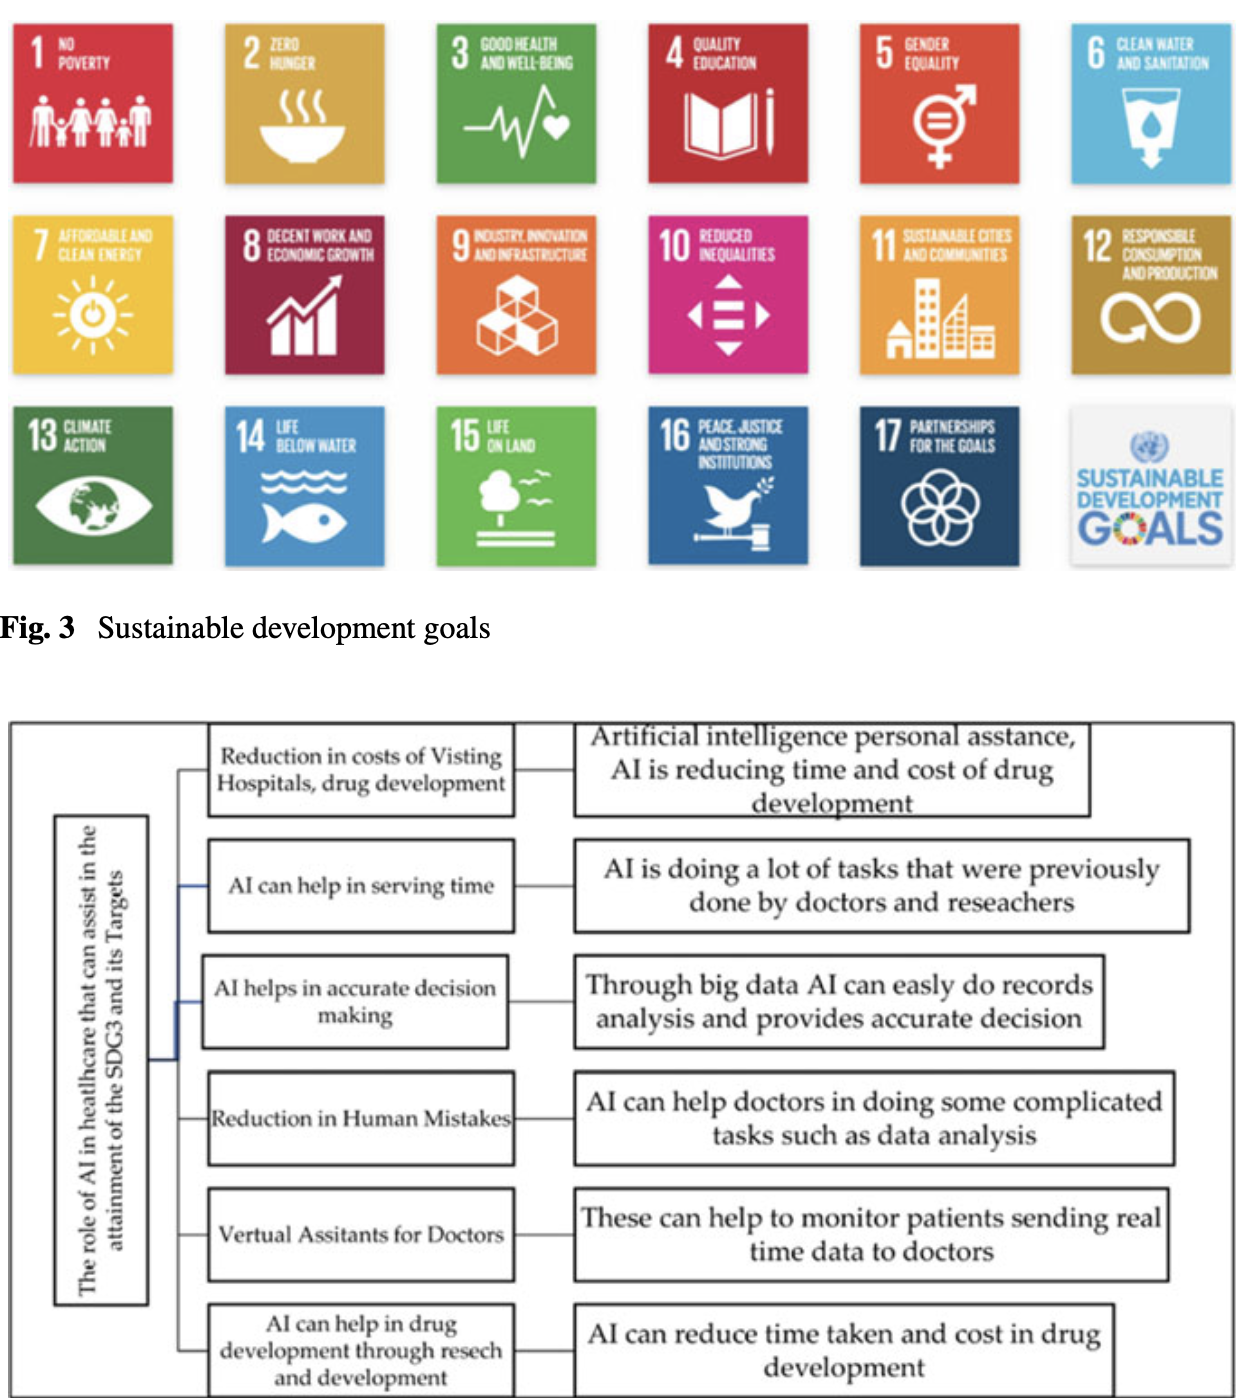
\includegraphics[width=1\textwidth]{figures/SR0023US23/fig2.png}
        \caption{Goals and AI possibilities from \cite{x101}.}
        \label{fig2:SR0023US23}
    \end{figure}

    \textbf{Page 5-10 (Literature Review):}
    Describtion of different implementations of AI around the globe. General understanding.
    \begin{figure}[H]
        \centering
        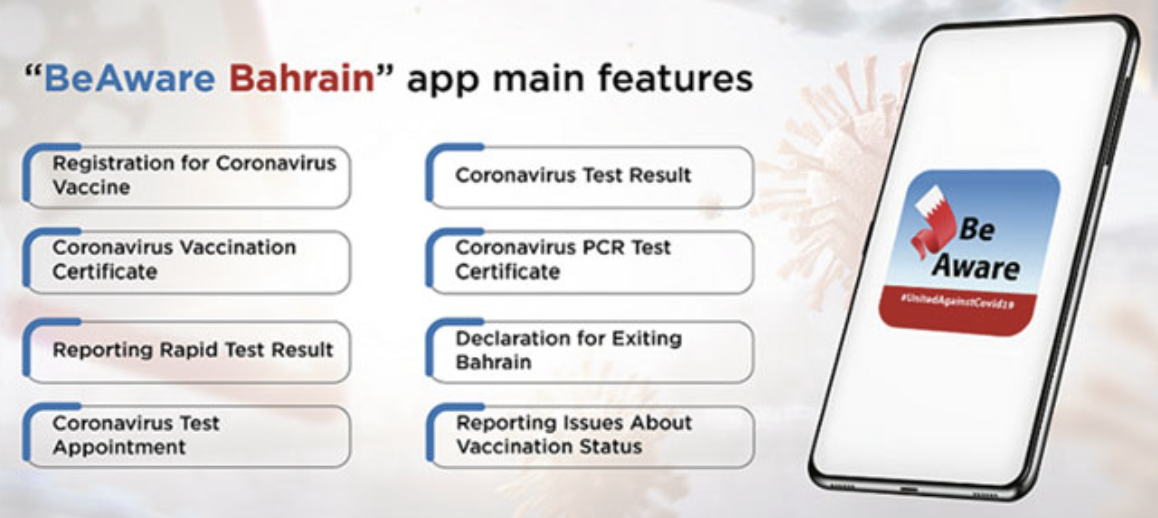
\includegraphics[width=1\textwidth]{figures/SR0023US23/fig1.png}
        \caption{BeAware App in Bahrain from \cite{x101}.}
        \label{fig1:SR0023US23}
    \end{figure}
    
    \textbf{Page 10-15 (Scope of the Study):}
    Automatic control of donning and doffing policy complience from staff members. Description of AI enhanced CT scanse recognition in Netherlands and Germany: comperison and potential implementation in Bahrain.
    \begin{figure}[H]
        \centering
        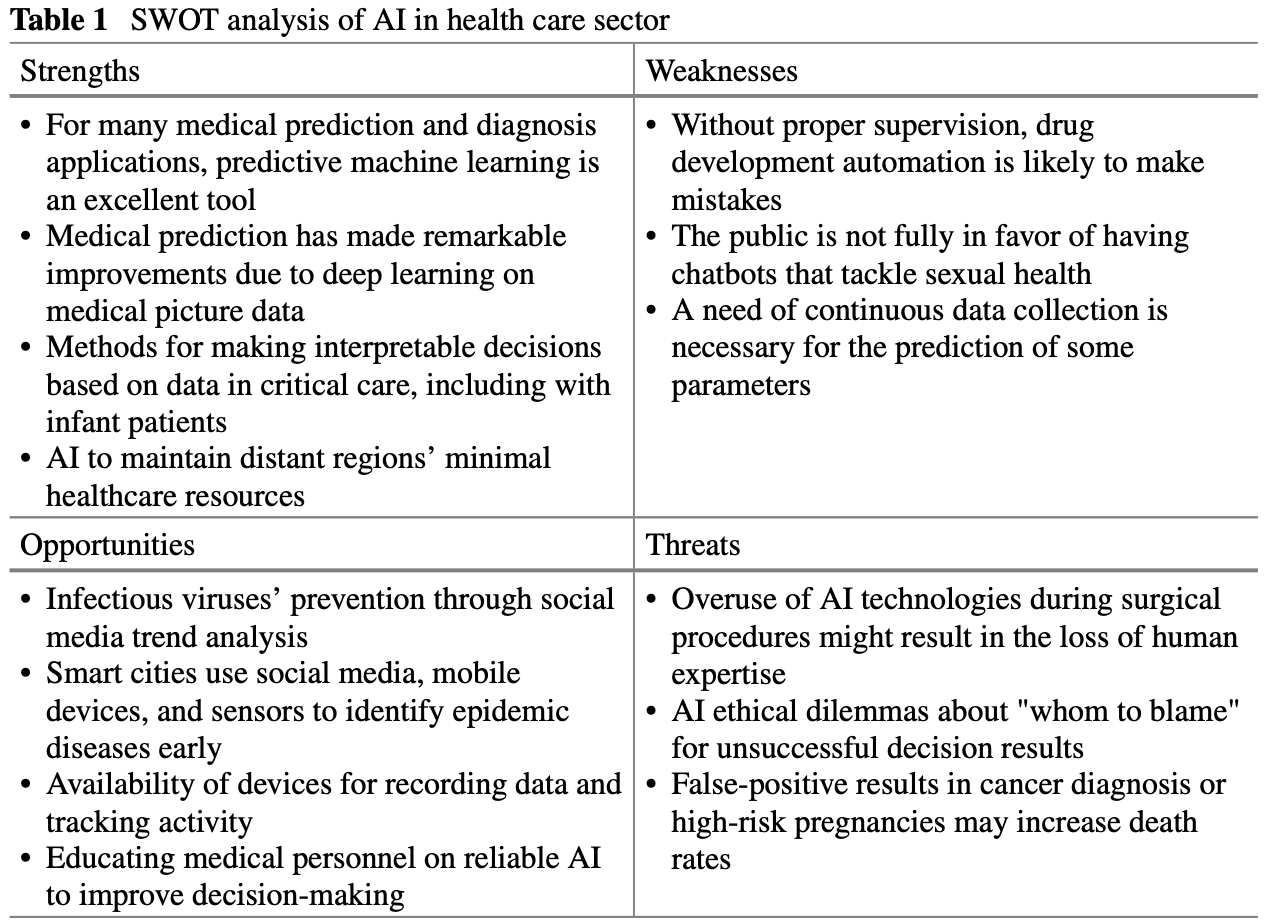
\includegraphics[width=1\textwidth]{figures/SR0023US23/fig3.png}
        \caption{SWOT pros and cons from \cite{x101}.}
        \label{fig3:SR0023US23}
    \end{figure}

    \textbf{Page 15-16 (Conclusion):}
    Bahrain has great acheavements in AI sector but there is also room for improvement.
    
    \textbf{Page 16 (Recommendations):}
    (1) Robotic AI enhancement;
    (2) AI in mental health sphere;
    (3) Patient delivery services;
    (4) Radiology - scans illness detection.

    \textbf{Page 16-17 (Research Limitations and Future Work):}
    \underline{Limitations}:
    (a) Comparison with just few countries;
    (b) AI in Healthcare sector;
    (c) Introduction and lit. review only;
    (d) smth, smth SDG ???;
    (e) smth, smth marketing ???.
    \underline{Future Work}:
    (I) Integrating new AI techniques in Bahrain;
    (II) Overview research in more countries;
    (III) smth, smth workers ???.